\documentclass[a4paper,12pt,oneside,openright,titlepage]{book}
\usepackage[utf8]{inputenc}
\usepackage[T1]{fontenc}
\usepackage[english]{babel}

\usepackage{amsmath}
\usepackage{amsfonts}
\usepackage{amssymb}
\usepackage{latexsym} 

\usepackage{graphicx}
\graphicspath{ {./images/} }
\usepackage{color}
\usepackage{textcomp}
\usepackage{etoolbox}    
\usepackage{listings}
\usepackage[pdftex]{hyperref}
\usepackage{url}
\usepackage[numbers]{natbib} 

%%% Taken from https://www.entwickler-ecke.de/topic_C+Darstellung+fuer+Latex+listings_100839,0.html

\usepackage{color}
\usepackage{listings}    
\usepackage{courier}


%%% Define Custom IDE Colors %%%
\definecolor{arduinoGreen}    {rgb} {0.17, 0.43, 0.01}
\definecolor{arduinoGrey}     {rgb} {0.47, 0.47, 0.33}
\definecolor{arduinoOrange}   {rgb} {0.8 , 0.4 , 0   }
\definecolor{arduinoBlue}     {rgb} {0.01, 0.61, 0.98}
\definecolor{arduinoDarkBlue} {rgb} {0.0 , 0.2 , 0.5 }

%%% Define Arduino Language %%%
\lstdefinelanguage{Arduino}{
  language=C++, % begin with default C++ settings 
%
%
  %%% Keyword Color Group 1 %%%  (called KEYWORD3 by arduino)
  keywordstyle=\color{arduinoGreen},   
  deletekeywords={  % remove all arduino keywords that might be in c++
break, case, override, final, continue, default, do, else, for, if, return, goto, switch, throw, try, while, setup, loop, export, not, or, and, xor, include, define, elif, else, error, if, ifdef, ifndef, pragma, warning,HIGH, LOW, INPUT, INPUT_PULLUP, OUTPUT, DEC, BIN, HEX, OCT, PI, HALF_PI, TWO_PI, LSBFIRST, MSBFIRST, CHANGE, FALLING, RISING, DEFAULT, EXTERNAL, INTERNAL, INTERNAL1V1, INTERNAL2V56, LED_BUILTIN, LED_BUILTIN_RX, LED_BUILTIN_TX, DIGITAL_MESSAGE, FIRMATA_STRING, ANALOG_MESSAGE, REPORT_DIGITAL, REPORT_ANALOG, SET_PIN_MODE, SYSTEM_RESET, SYSEX_START, auto, int8_t, int16_t, int32_t, int64_t, uint8_t, uint16_t, uint32_t, uint64_t, char16_t, char32_t, operator, enum, delete, bool, boolean, byte, char, const, false, float, double, null, NULL, int, long, new, private, protected, public, short, signed, static, volatile, String, void, true, unsigned, word, array, sizeof, dynamic_cast, typedef, const_cast, struct, static_cast, union, friend, extern, class, reinterpret_cast, register, explicit, inline, _Bool, complex, _Complex, _Imaginary, atomic_bool, atomic_char, atomic_schar, atomic_uchar, atomic_short, atomic_ushort, atomic_int, atomic_uint, atomic_long, atomic_ulong, atomic_llong, atomic_ullong, virtual, PROGMEM, Serial, Serial1, Serial2, Serial3, SerialUSB, Keyboard, Mouse,abs, acos, asin, atan, atan2, ceil, constrain, cos, degrees, exp, floor, log, map, max, min, radians, random, randomSeed, round, sin, sq, sqrt, tan, pow, bitRead, bitWrite, bitSet, bitClear, bit, highByte, lowByte, analogReference, analogRead, 
analogReadResolution, analogWrite, analogWriteResolution, 
attachInterrupt, detachInterrupt, digitalPinToInterrupt, delay, delayMicroseconds, digitalWrite, digitalRead, interrupts, millis, micros, noInterrupts, noTone, pinMode, pulseIn, pulseInLong, shiftIn, shiftOut, tone, yield, Stream, begin, end, peek, read, print, println, available, availableForWrite, flush, setTimeout, find, findUntil, parseInt, parseFloat, readBytes, readBytesUntil, readString, readStringUntil, trim, toUpperCase, toLowerCase, charAt, compareTo, concat, endsWith, startsWith, equals, equalsIgnoreCase, getBytes, indexOf, lastIndexOf, length, replace, setCharAt, substring, toCharArray, toInt, press, release, releaseAll, accept, click, move, isPressed, isAlphaNumeric, isAlpha, isAscii, isWhitespace, isControl, isDigit, isGraph, isLowerCase, isPrintable, isPunct, isSpace, isUpperCase, isHexadecimalDigit, 
                }, morekeywords={   % add arduino structures to group 1\\
  break, case, override, final, continue, default, do, else, for, if, return, goto, switch, throw, try, while, setup, loop, export, not, or, and, xor, include, define, elif, else, error, if, ifdef, ifndef, pragma, warning,}, 
% 
%
  %%% Keyword Color Group 2 %%%  (called LITERAL1 by arduino)
  keywordstyle=[2]\color{arduinoBlue},   
  keywords=[2]{   % add variables and dataTypes as 2nd group  
HIGH, LOW, INPUT, INPUT_PULLUP, OUTPUT, DEC, BIN, HEX, OCT, PI, HALF_PI, TWO_PI, LSBFIRST, MSBFIRST, CHANGE, FALLING, RISING, DEFAULT, EXTERNAL, INTERNAL, INTERNAL1V1, INTERNAL2V56, LED_BUILTIN, LED_BUILTIN_RX, LED_BUILTIN_TX, DIGITAL_MESSAGE, FIRMATA_STRING, ANALOG_MESSAGE, REPORT_DIGITAL, REPORT_ANALOG, SET_PIN_MODE, SYSTEM_RESET, SYSEX_START, auto, int8_t, int16_t, int32_t, int64_t, uint8_t, uint16_t, uint32_t, uint64_t, char16_t, char32_t, operator, enum, delete, bool, boolean, byte, char, const, false, float, double, null, NULL, int, long, new, private, protected, public, short, signed, static, volatile, String, void, true, unsigned, word, array, sizeof, dynamic_cast, typedef, const_cast, struct, static_cast, union, friend, extern, class, reinterpret_cast, register, explicit, inline, _Bool, complex, _Complex, _Imaginary, atomic_bool, atomic_char, atomic_schar, atomic_uchar, atomic_short, atomic_ushort, atomic_int, atomic_uint, atomic_long, atomic_ulong, atomic_llong, atomic_ullong, virtual, PROGMEM,},  
% 
%
  %%% Keyword Color Group 3 %%%  (called KEYWORD1 by arduino)
  keywordstyle=[3]\bfseries\color{arduinoOrange},
  keywords=[3]{  % add built-in functions as a 3rd group
                Serial, Serial1, Serial2, Serial3, SerialUSB, Keyboard, Mouse,
                },      
%
%
  %%% Keyword Color Group 4 %%%  (called KEYWORD2 by arduino)
  keywordstyle=[4]\color{arduinoOrange},
  keywords=[4]{  % add more built-in functions as a 4th group
abs, acos, asin, atan, atan2, ceil, constrain, cos, degrees, exp, floor, log, map, max, min, radians, random, randomSeed, round, sin, sq, sqrt, tan, pow, bitRead, bitWrite, bitSet, bitClear, bit, highByte, lowByte, analogReference, analogRead, 
analogReadResolution, analogWrite, analogWriteResolution, 
attachInterrupt, detachInterrupt, digitalPinToInterrupt, delay, delayMicroseconds, digitalWrite, digitalRead, interrupts, millis, micros, noInterrupts, noTone, pinMode, pulseIn, pulseInLong, shiftIn, shiftOut, tone, yield, Stream, begin, end, peek, read, print, println, available, availableForWrite, flush, setTimeout, find, findUntil, parseInt, parseFloat, readBytes, readBytesUntil, readString, readStringUntil, trim, toUpperCase, toLowerCase, charAt, compareTo, concat, endsWith, startsWith, equals, equalsIgnoreCase, getBytes, indexOf, lastIndexOf, length, replace, setCharAt, substring, toCharArray, toInt, press, release, releaseAll, accept, click, move, isPressed, isAlphaNumeric, isAlpha, isAscii, isWhitespace, isControl, isDigit, isGraph, isLowerCase, isPrintable, isPunct,isSpace, isUpperCase, isHexadecimalDigit,},      
%
%
  %%% Set Other Colors %%%
  stringstyle=\color{arduinoDarkBlue},    
  commentstyle=\color{arduinoGrey},    
%          
%   
  %%%% Line Numbering %%%%
   numbers=left,                    
  numbersep=5pt,                   
  numberstyle=\color{arduinoGrey},    
  %stepnumber=2,                      % show every 2 line numbers
%
%
  %%%% Code Box Style %%%%
  breaklines=true,                    % wordwrapping
  tabsize=2,         
  basicstyle=\ttfamily  
}
\usepackage{courier, color, listings}

\definecolor{Green}{rgb}{0, 0.3, 0}
\definecolor{DarkCyan}{rgb}{0, 0.545, 0.545}
\definecolor{Navy}{rgb}{0, 0, 0.5}
\definecolor{Teal}{rgb}{0, 0.5, 0.5}
\definecolor{DarkGray}{gray}{0.66}
\definecolor{Olive}{rgb}{0.5, 0.5, 0}
\definecolor{Pink}{rgb}{1.0, 0.75, 0.8}
\definecolor{DeepPink}{rgb}{1, 0.08, 0.58}
\definecolor{Brown}{rgb}{0.65, 0.165, 0.165}
\definecolor{DarkViolet}{rgb}{0.58, 0, 0.83}
\definecolor{SaddleBrown}{rgb}{0.55, 0.27, 0.07}
\lstdefinelanguage{CSharp}
{
 morecomment = [l]{//}, 
 morecomment = [l]{///},
 morecomment = [s]{/*}{*/},
 morestring=[b]", 
 morestring=[b]',
 basicstyle=\footnotesize\ttfamily,
 commentstyle=\color{Green}\textit,
 stringstyle=\color{blue},
 sensitive = true,
  morekeywords=[1]{this, base},
  keywordstyle=[1]\bfseries,
  morekeywords=[2]{as, is, new, sizeof, typeof, true, false, stackalloc, ArduinoData, Key},
  keywordstyle=[2]\color{DarkCyan}\bfseries,
  morekeywords=[3]{else, if, switch, case, default,
  do, for, foreach, while, in},
  keywordstyle=[3]\color{blue}\bfseries ,
  morekeywords=[4]{break, continue, goto, return,
  yield, partial, global, where},
  keywordstyle=[4]\color{Navy},
  morekeywords=[5]{try, throw, catch, finally},
  keywordstyle=[5]\color{Teal}\bfseries,
  morekeywords=[6]{checked, unchecked},
  keywordstyle=[6]\color{DarkGray}\bfseries,
  morekeywords=[7]{fixed, unsafe},
  keywordstyle=[7]\color{Olive},
  morekeywords=[8]{bool, byte, sbyte, char, short, ushort, int, uint, long, ulong, float,
  double, decimal, enum, struct},
  keywordstyle=[8]\bfseries\color{blue},
  morekeywords=[9]{class, interface, delegate, object, string,
  void},
  keywordstyle=[9]\color{red},
  morekeywords=[10]{explicit, implicit, operator},
  keywordstyle=[10]\color{Pink}\bfseries,
  morekeywords=[11]{params, ref, out},
  keywordstyle=[11]\bfseries\color{DeepPink},
  morekeywords=[12]{private, protected, internal, public},
  keywordstyle=[12]\bfseries\color{blue},
  morekeywords=[13]{abstract, const, event, var, override, virtual, volatile, extern, readonly, sealed, static},
  keywordstyle=[13]\color{Brown},
  morekeywords=[14]{namespace, using},
  keywordstyle=[14]\bfseries\color{Green},
  morekeywords=[15]{lock},
  keywordstyle=[15]\color{DarkViolet},
  morekeywords=[16]{get, set, add, remove},
  keywordstyle=[16]\color{SaddleBrown},
  morekeywords=[17]{null, value},
  keywordstyle=[17]\bfseries,
}
\lstset{tabsize=4,showstringspaces=false, numberstyle=\tiny, stepnumber=2, numbersep=5pt}
\newenvironment{dedication}%
{\cleardoublepage\addcontentsline{toc}{chapter}{Dedication}\null\vfill\begin{flushright}}%
{\end{flushright}\vfill\null}

\newenvironment{abstract}%
{\cleardoublepage\addcontentsline{toc}{chapter}{Abstract}\null\vfill\begin{center}%
\bfseries\abstractname\end{center}}%

\title{Automatic Gardening System}
\author{Kristmund Ryggstein and Hergeir Winther Lognberg \\ University of the Faroe Islands\\}

\begin{document}
\frontmatter
\maketitle

\begin{abstract}
Vit vóru bidnir um at gera eina KT Verkætlan, og í tí sambandinum valdu vit at gera ein automatiskan urtapott, sum vísti dátu um urtapottin á einari heimasíðu. Hesin urtapotturin kann máta ljós, fugt, hita og kann eisini pumpa vatn í urtapottin. Hetta valdu vit, tí tað her henda nógv ting á Sandoynni, har vit eru frá, viðvíkjandi gróðrarvirksemi. Vit brúka ein Arudino Uno sum miðstøð fyri allar sensorarnar. Øll dátu vera send á ein servara gjøgnum eitt ESP8266-05 Wifi modul. Á hesum servara ber tað til at lesa dátu um urtapottir, ið eru knýttir at einum brúkara.

\end{abstract}

\cleardoublepage\addcontentsline{toc}{chapter}{Contents}
\tableofcontents

\chapter{Foreword}

We believe that the project has been challenging but also incredible rewarding, because this is the largest project we both have worked on so far. Our version control has been Github, and all our code and project description is available there.
\begin{itemize}
\item\href{https://github.com/Hergeirs/Arduino2/tree/master/FWG7RQ3IRXT1DFL}{Arduino code}
\item \href{https://github.com/Hergeirs/Arduino-Web}{Web Code}
\item \href{https://github.com/Hergeirs/Arduino-Report}{IT Report}
\end{itemize}
We've also attached code we deemed important in the appendix, because it is easier to refer it from there. The code from the Arduino projects are the cpp files and the Arduino ino file. The report is in two parts, one is the arduino part and one is the webserver part.
\section*{Acknowledgement}
We want to thank The University of The Faroe Islands for providing us with the materials provided to us from the beginning, and to thank them for providing us with the funds to procure new materials. We also want to thank Benadikt Joensen for guiding  and teaching us the more electrical side of things in our project.
\addcontentsline{toc}{section}{Acknowledgement}

\mainmatter
\chapter{Introduction}

The purpose of this report is to document our project and the process of developing it. The purpose of the project is to create a system that has basic gardening capabilities, and is able to procure data from its plants and present them.

We have chosen to work with automatic a gardening system because it has some tasks, what we believe can be easily automated. There has been an increasing interest on Sandoy in trying to grow and sell more vegetables on the islands. That grown interest in thanks to initiatives such as "Veltan" and "Eplafestivalurin". Trying to be self-sufficient with regards to food produce is something we agree upon, and that's were we think that our modest electronic gardening project fits well with that philosophy, and will be an interest for those, who want to try to be more self-sufficient.

We need to measure at least light, moisture, and temperature in order for in to be a valid gardening system. We need a method to send data and something to present those data.
\addcontentsline{toc}{section}{Introduction}

\chapter{Setup}
The Arduino Uno, TMP36GZ heat sensor, LDR, other resistors and the cables which we use in this project, was provided by the one responsible by the course. We used at the start a FC28 moisture sensor, but it generally uses DC current which means that it corrodes quickly because of electrolysis in the soil and alters the soil composition which could potentially damage the plant. That would also eventually lead to tainted readings. We changed it to use an AC pulse that can be seen in figure, but we decided to opt for a Capacitive Soil Moisture Sensor V1.2 that is Corrosion Resistant. The FC28 sensor can be seen in \ref{fig:resistive} and the capactive sensor can be seen in the section about it.

\section{Arduino}
Arduino is an open-source electronics platforms which is based on user-friendly software and hardware components\cite{ArduinoIntroduction}. It can read outputs from these components e.g. readings from sensors, and it can give input to these sensors.

We worked on an Arduino Uno. It is a microcontroller board. It has 14 digital i/o pins. They can be located on the board right next to the text \textit{DIGITAL}. Six of those pins can be used as Power Width Modulation, shortened as PWM, outputs. Those pins are the ones who have a ~ next to their ascribed numbers. It has six analog pins. It then has five different kinds of power pins. We only use the GND and the 5V and 3.3V pins. The 5V and 3.3 pins output a 5V and 3.3V from the regulator on the board which can be used to power different hardware components. The 3.3V pins has a maximum current draw of 50mA. GND stands for ground, and serves as the common return path for current from the different hardware components in our Arduino system. A graphic representation of it can be viewed in section 2.2.1. 

\subsection{Arduino Main}
The code for where the Arduino setup and loop are in \ref{list:ArduinoMain}. The first lines are inclusions of sensors and the SoftwareSerial library which is used to connect the ESP8266-05 module. The next block is where we define our internet properties and which port to communicate through. The third block is our declarations i.e. what digital pins on the Arduino are attached to the Rx and Tx pins for the wifi module then we use that first declaration to setup the ESP8266 wifi with the baudrate 115200. Setup method sets the Arduino up for the loop() method. The while loop tries to establish a connection to an access point with the predefined SSID and PASSWORD. If that succeeded, then it prints to the the console that it was a success and breaks out of the loop, otherwise it prints that it failed. All Serial.print functions are used as debugging tools, so that we are able tell if something is wrong or not. The loop will try to reconnect to the wifi every twentieth second. That is done so that we don't need to restart the Arduino every time something goes wrong. The next loop tries to establish a TCP connection to the Webserver. TCP stands for Transmission Control Protocol and it is a standard for how to establish and maintain a connection for how application programs can transmit data to each other over IP. 

Data is a struct which holds all our information which the sensors reads. Its a way for us to structure our data. Water never gets used, and it was supposed to say how much water was in a tank. It never got used because its the least important thing in our project, and we wanted to focus on finishing the web server.

Package is also a struct, and it creates a union of data values and a unsigned int8\_t array of bytes with the size nine. It takes nine bytes because that is that accumulated max size of all the variables in the Data struct.

Datahandler is class that populates that Package. First it creates an integer constant and assigns it to one, then it creates object instances of our sensors. CapacitiveMoistureSensor is set to digital pin four and analog pin two, TemperatureSensor is set to eight and one etc. 

PopulatePackage() does as the name implies. First it creates a variable reference of type Data and assigns it the package in line 81, then it takes the values in that package and assigns it the DataHandler id, and what the sensors are reading. Water gets assigned a random number. getPackage() calls the populatePackage() method and returns a reference to that package.

loop() is the method that is constantly running, when the Arduino is turned on. That means that for every iteration of the loop, it creates a Package and assigns it with values from populatePackage, and tries to send it to the webserver. First the actual data is supplied to Wifi.Send, then the size of the packace. There's a five seconds delay for every iteration.

\section{Moisture Sensors}
\subsection{FC28}
Our intention was to use the Arduino to induce an alternating current through the sensor. To simplify things, we circumvented the circuit of FC-28 such that we connected directly to the pins on the sensor. To alternate the current, we first emit 5V from pin 12 and set pin 13 to low (0V) for 1 ms then we take a reading through the analog pin A0. Then we flip the pin 12 and 13 ( 5V from pin 13 ) for the same amount of time. This should somewhat remedy the problems of electrolysis by shifting the ions back and forth between the moisture sensor pins, instead of just letting them congest at one pin. The chip had to be removed so that it could use AC.
The setup can be seen below.

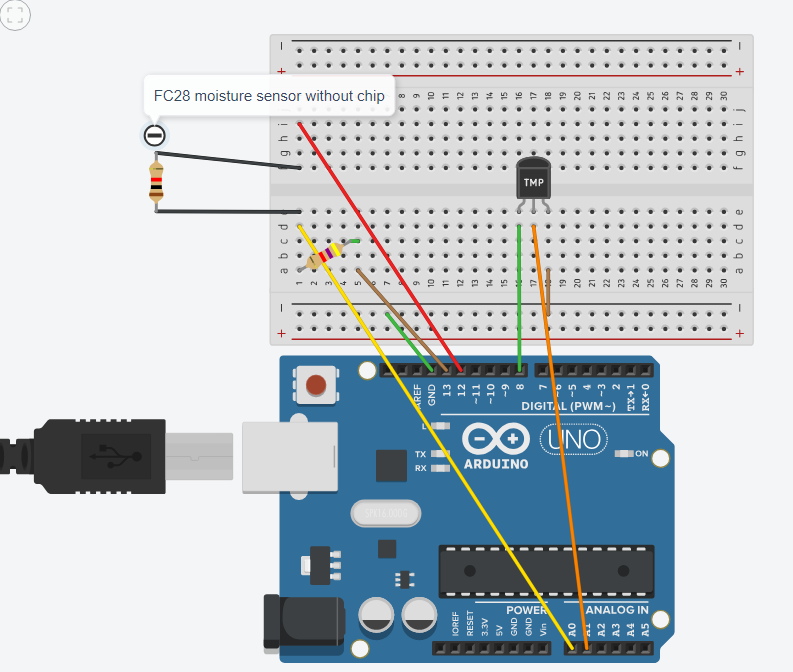
\includegraphics[scale = 0.50]{FC-28-Diagram.PNG}\label{graph:capacitive}

The resistor in the circuit helps increase the amount of current entering the analog sensor. Without it about half the current would go in the pin 13 when the measurement occurs. We are therefor able to steer the range of current entering the analog input. The left left leg is connected to 8 digital pin, the middle leg is connected to A1 pin, and the third leg is connected to -18 on the breadboard which is then connected to the ground pin on the Arduino.  

\subsection{Capacitive Soil Moisture Sensor v1.2}
\begin{center}
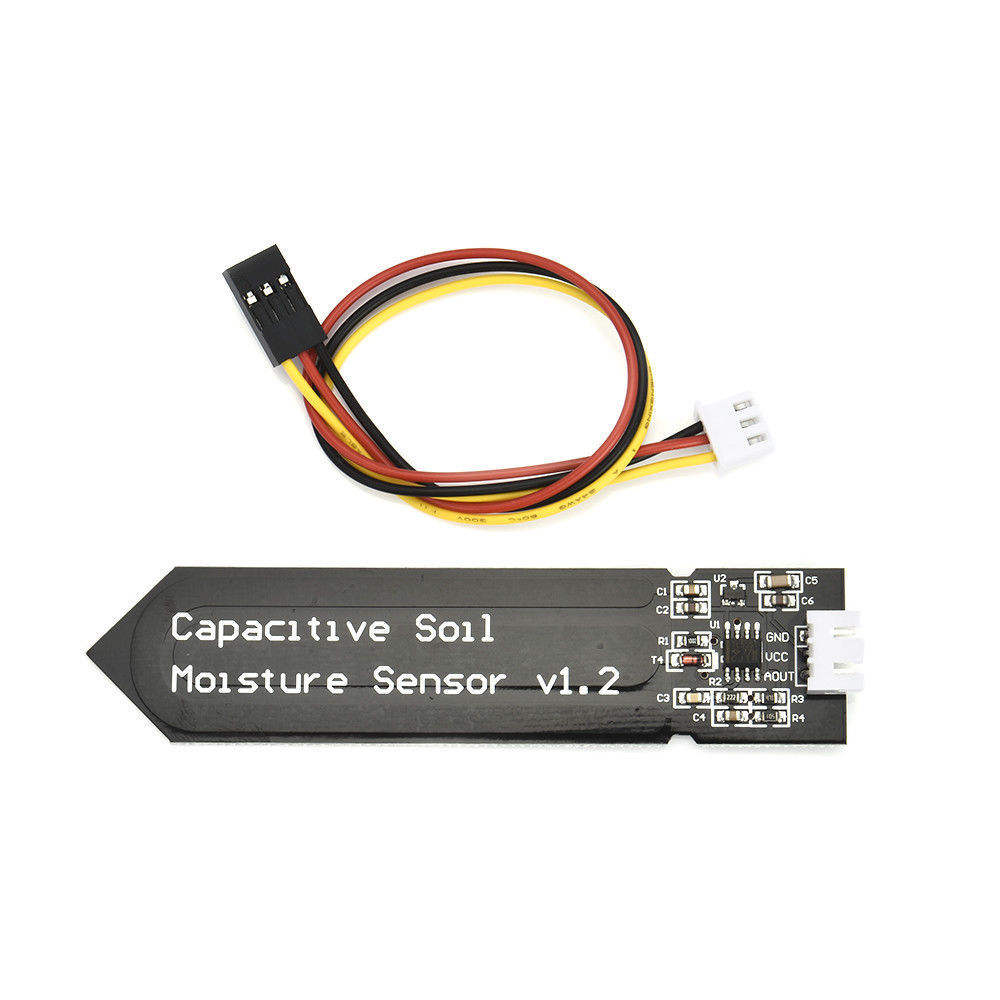
\includegraphics[scale=0.20]{capacitive-sensor}
\end{center}

We looked at reviews, and this one seemed to be the most corrosion resistant of the ones we looked at. It is made by corrosion resistant material, so it has a higher lifetime than the other sensor. It measures moisture, or rather the ions in the soil, by reading the capacitance between two plates in the sensor. It has lesser range than the other one, as it measures air values as 555 and completely submerged as 280. We thought the minimized range wouldn't worsen our readings, and the benefit from increased lifetime far outweighed the potential range.

\begin{lstlisting}[language=Arduino]
uint8_t CapacitiveMoistureSensor::readPercent(uint16_t val)
{
     /* 555 is the value for moisture in the air
	 // 288 is the value for when the sensor is submerged in water
	  then sett 555 to be 0%, 288 to be 100%, and map the percent between them */
	
	val = constrain(val,280,555);
	double valPercent = map (val, 555, 280, 0, 100);

	return valPercent;
}

\end{lstlisting}
readPercent takes the read value from the analog read, and converts it to a percent that is mapped between air- and water value. Line 7 sets a constrain on val variable which says that it can't be more than 555 and not less than 280. Line 8 creates a new variable, which is val parameter mapped as a percentage between 555 and 280 where 555 is 0\% and 280 is 100\%. That number is then returned when the method is called.

\begin{lstlisting}[language=Arduino]
uint8_t CapacitiveMoistureSensor::read()
{
	digitalWrite(dPin,HIGH);
	delay(1000);
    uint16_t val = analogRead(aPin);
	digitalWrite(dPin,LOW);
    return readPercent(val);
}
\end{lstlisting}

This method reads the output from the capacitive sensor. digitalWrite(dPin, HIGH) starts the sensor. dPin is the the digital pin in which the sensor is connected to the Arduino. delay(1000) pauses the code at one second, then it initalized the val variable through analogRad(aPin), where aPin is the analog pin which the sensor is connected. Then the method calls the above readPercent(val) method,which returns the converted number as a percentage.

\section{Temperature Sensor}
\subsection{TMP-36 Sensor}
\begin{center}
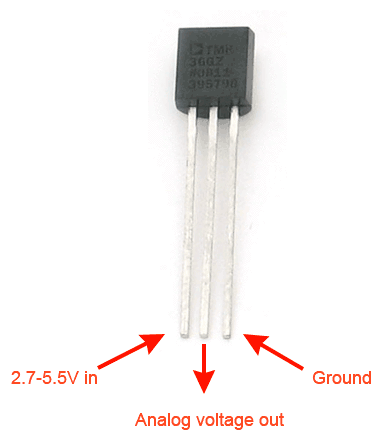
\includegraphics[scale=0.8]{TMP-36}
\end{center}


We used the TMP36 temperature sensor, as it was supplied to use by the course administrators and that it suits our purpose. The TMP36 is fairly simple. It can measure degrees from -40\textdegree{}C to \textdegree{125}C, where it has a precision\cite{tmpTutorial} of $\pm2$\textdegree{}C. It works as a diode so when it changes temperature, it then its voltage changes accordingly. The sensor measures the small change and outputs an analog output based on it, so its possible to calculate the temperature according to that output. 
The sensor's collector pin is attached to the 8 digital pin, the gate to the analog input A1 and the third leg is the ground.
We use a readCelcius() method from the Temperature Class, and it can be seen below.
\begin{lstlisting}[language=Arduino]
const int8_t TemperatureSensor::readCelsius()
{
    digitalWrite(triggerPin, HIGH);
    delayMicroseconds(200);
    uint16_t reading = analogRead(readPin);
    digitalWrite(triggerPin, LOW);
    // converting that reading to voltage, for 3.3v arduino use 3.3
    double voltage = reading * 5.0; // * 0.0009775171;
    voltage /= 1024.0;
    return round((voltage - 0.5) * 100);
}
\end{lstlisting}
digitalWrite(triggerPin, HIGH) sends a pulse to the sensor which starts it, then delayMicroseconds() delays the program, so that the sensor waits while the sensor is activated. Then reading = analogRead(readPind) reads the output from the sensor. The output from it, is converted to voltage by multiplying it with five. That is then divided by 1024 to find the percentage of the analog read, because the Arduino outputs between 0 and 1023, where 0 is not voltage and 1023 is 5V. Five is then subtracted from that, and then that result is multiplied with 100 to convert it from mV to degrees. Five is subtracted from the reading because we want it so that 0V corresponds to -50\textdegree{}C. 

\section{Light Sensor}
\subsection{LDR Resistor}

\begin{center}
	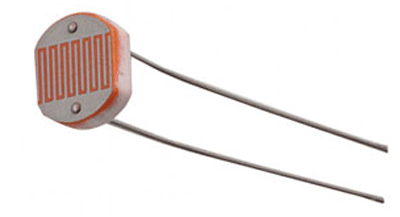
\includegraphics[scale=0.80]{LDR-Resistor}
\end{center}


We use a LDR Resistor to detects the level of light in the room. The resistor changes its resistance based on how much light is in the room. If the room is unlit then the resistor will have a resistance of a few ohms, but will decrease if the room gets lighter. It's not ideal for our purpose because it's not very sensitive, and that it needed to be calibrated. We chose it because it was available and that we wanted to focus on the webserver and other areas of the project.

\section{Water Pump}
\subsection{Water Pump}
\begin{center}
	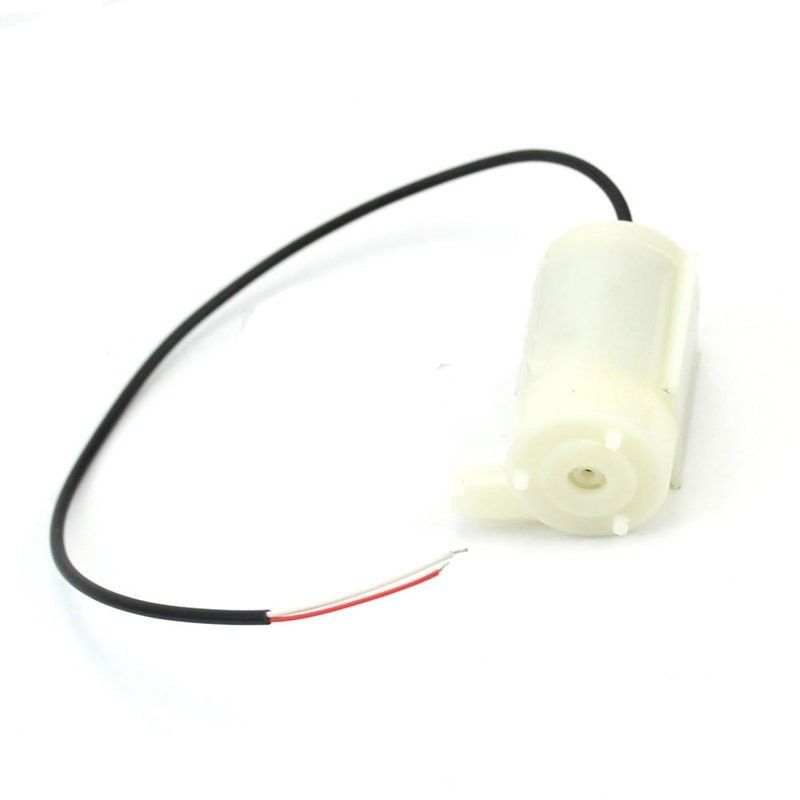
\includegraphics[scale=0.3]{Water-Pump}
\end{center}

Our water pump is said to have a flow rate of 80-120L\\H. We haven't tested if that is correct, but our tests to see if it worked deemed that it's pumping flow rate is more than enough for our use. It uses a DC current 2.5-6V. The rest of the product description is in \ref{fig:pump description}. Its tube was bought in the local Pet store, and was glued on the facing  left in the picture.

\section{Wifi Module}
\subsection{ESP8266-05}
\begin{center}
	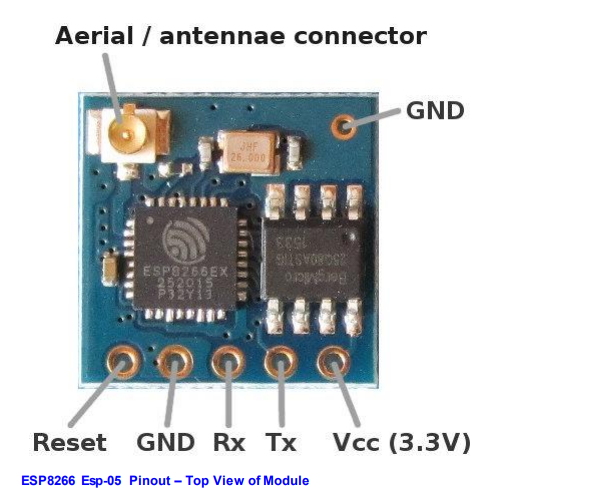
\includegraphics[scale=0.3]{ESP8266}
\end{center}

The ESP8266-05 wifi module was the hardest to work with. We initially bought an ESP8266-01\ref{fig:ESP}, but that was even more complex to work with, because it had 8 pins, and the distance between each pin on the module was so small that we couldn't properly solder it. We then bought the 05 version which was much easier to solder. A picture is attached of the module in \ref{fig:ESP}. We don't use the antennae nor the upper GND pin. We have a problem with the module in that the Arduino UNO 3.3V supply has inadequate current capabilities to power it. It still works but we get occasional garbage data from the packages sent sent from the module. Garbage transmissions seem to increase the longer the module is in use. It's possible to use an alternate 3.3V supply rather than the one from the Arduino but we didn't look into it, as it would take focus from some of the other work needed in the development. We used an \href{https://github.com/Hergeirs/Arduino2/blob/master/FWG7RQ3IRXT1DFL/ESP8266.h}{ESP8266 library} which  has the methods send(), joinAP which we use.

\chapter{Website}
\section*{Webserver}
We chose to work with Microsoft's ASP.NET Core which is an open-source cross-platform framework for building cloud-based and internet-connected applications. We chose this framework because we were familiar with it through the course 5022.16 Web Applications: ASP.NET with C\# which we had right before this course. It is something both collaborators in this project like to use. 

\section{Hosting}
We initially wanted to host the webserver on Microsoft's Azure which all university students get access to through Microsoft's student offer. We quickly found out that it didn't work for us, because we couldn't connect to any of its ports. 

\section{Login}
We found out that .Net Core has something called Identity Core\cite{Identity} which handles the login for an ASP.NET Core application. The user can create a membership for the application by using his or she's Facebook, Twitter, Microsoft, or Google login credentials. We could have added the other options, but we deemed it unnecessary as most faroese that would be willing to use a system such ours will most likely have a Facebook account. It's also possible to login with a regular email.

\begin{lstlisting}[language=CSharp] 
services.AddAuthentication().AddFacebook(facebookOptions =>
{
	facebookOptions.AppId =
			 Configuration["Authentication:Facebook:AppId"];
	facebookOptions.AppSecret =
			 Configuration["Authentication:Facebook:AppSecret"];
});
\end{lstlisting}

This code block adds Facebook authentication to our login service. facebookOptions.AppId and facebookOptions.AppSecret are plugins from chrome which had to be created in Chrome to support facebook login for our project. We found the tutorial for it on \cite{FacebookLogin} which is Microsoft's support page for Facebook external login. The idea with the login functionality is that plants can be attached to users in our system, and that he is able to view data about his plants on the website.

\section{Project E.Garden Structure}
Our .Net Core project is divided into three parts. It's good practice to have all business logic i.e. models that represents plants, users, and Arduino Data in a separate class library from the main program. It's done so the project is decoupled, and so that the classes can be inc. First part is the Model folder where the classes are and can be seen in \ref{list:Models}. ApplicationUser inherits from User, because that makes it so that the properties from ApplicationUser gets added to AspNetUsers in the database. That is a functionality of the previously mentioned Identity. 


One part of the repository library is a folder that contains the skeleton i.e. interfaces for our business handling, then the implementation of those interfaces is located in the Concrete folder. This means that the EFPlantRepository model inherits from IPlantRepository, and then specifies what the methods UserPlants() and SavePlants() should do. These repositories are then initialized in the file Startup.cs, specifically the ConfigureServices(IServiceCollection services) method. It's initialized with something called Dependency Injection\cite{DependencyInjection}


\label{list:DpInjection}
\begin{lstlisting}[caption={Dependency Injection}, language=CSharp]
	services.AddScoped<IApplicationUserAccessor, ApplicationUserAccessor>();
	services.AddScoped<IPlantRepository, EFPlantRepository>();
    services.AddScoped<IArduinoDataRepository, EFArduinoDataRepository>();
\end{lstlisting}

This initializes at run time all instances of those three interfaces as the specified implementation. AddScoped establishes the lifetime of the services, and scoped means that it is created once per request. The code for the interfaces can be seen in \ref{list:Interfaces}. The implementations and the explanations for the interfaces can be seen below.

\begin{lstlisting}[caption={EFArduinoDataRepository Class}\label{list:Concrete EFArduinoDataRepository}, language=CSharp]
public class EFArduinoDataRepository : IArduinoDataRepository
{
	private readonly EGardenerContext _context;
        
	public EFArduinoDataRepository(EGardenerContext context)
	{
        _context = context;
	}
	public void SaveData(ArduinoData data)
	{
		var context = _context;
		var plants = context.Plants.Include(x => x.Datas);
	    var plant = plants.Single(x => x.PlantId == data.PlantId);
        var datas = plant.Datas;
        datas.Add(data);
		context.SaveChanges();
	}
}
\end{lstlisting}

It has one private datamember called \_context of type EGardenerContext, which gets initialized in the EFArduinoDataRepository constructor. This context is the context between the models and their corresponding database entities. All the EFRepositories have this EGardenerContext. The SaveData(Arduino Data) is the actual implementation of the IArduinoDataReposistory. It takes an ArduinoData object as a parameter. First a new context variable is initialized, then a plant gets initialized by dotting into the context, and choosing a plant in the database that has a PlantId that corresponds to same id the data parameter has. A list of data gets initialized by assigning it to the data list in the newly created plant, and then the data parameter is added to that list. context.SaveChanges(); saves all the changes made.  This function is called in Observer's OnNext(ArduinoData value), and value gets saved there.


\begin{lstlisting}[caption={EFPlantRepository Class}\label{list:Concrete EFPlantRepository}, language=CSharp]
public class EFPlantRepository : IPlantRepository
{
	private readonly EGardenerContext _context;
    private readonly IApplicationUserAccessor _userAccessor;

	public EFPlantRepository(EGardenerContext context,
	IApplicationUserAccessoruserAccessor)
	{
		_context = context;
        _userAccessor = userAccessor;
	}

        
	public async Task<IEnumerable<Plant>> UserPlants()
	{

		var user = await _userAccessor.User;
            
		user = _context.Users.Include(x => x.Plants)
			.ThenInclude(x => x.Datas).Single(x => x.Id == user.Id);
            
            return user?.Plants ?? new List<Plant>();
	}

	public async Task SavePlant(Plant plant)
	{
		var user = await _userAccessor.User;
		var dbUser = await _context.Users.FindAsync(user.Id);

		plant.ApplicationUser = user;
		if (dbUser.Plants == null)
		{
	        dbUser.Plants = new List<Plant>();
        }
            
        dbUser.Plants.Add(plant);
        var amount = await _context.SaveChangesAsync();
	}
}
\end{lstlisting}
This class has a private field of type IApplicationUserAccessor called userAccessor which is used to access the users in the database. UserPlants() returns an asynchronous task that takes an IEnumerable<Plant>. IEnumerable is a C\#  build in interface which makes it easy to work with any kind of containers/lists. var user = await userAccessor.User initializes the variable with user that is currently logged in. User is then reassigned to the entity in the database that shares the same Id. Include(x => x.Plants) includes the plant list from the database user. ThenInclude then includes datas to each plant in the previous list. Single(x => x.Id == user.Id) finds the correct user. The method then either returns the user's plants or returns a new plant list. It returns the user plants when the user is not null and plants is also not null.

SavePlant(Plant plant) is an asynchronous method that stores a plant in the database.  It also initializes a user with the HttpContext, but it also creates one dbUser with one from the database. The dbUser is initialized similarly with how the user in UserPlants() got reassigned, and that is by locating it by user Id. The method suspends when it initialized those variables. The parameter, plant, then initializes its own user property to the user in this method. If db.User has an uninitialized plants property, then it gets initialized with a new empty one. The plant parameter then gets added to that plants property, and the \_context asynchronously saves the changes.
  
\subsection{Observer Pattern}
We decided to use Gang Of Four's observer pattern\cite{GoF}. We think that it fit well in our implementation of the communication between the Arduino and our Webserver. Microsoft have their own implementation of the pattern\cite{MicrosoftObserver} which we took inspiration from.
 
In short, the pattern is about having one class that has a list of dependencies which it notifies when there's a change.

\subsection{Observer}
Our provider is called Observer and implements the IObserver with ArduinoData in the template brackets. It can be seen in \ref{list:Observer}. That it implements the interface means that the class implements its own version of the methods
\begin{itemize}
\item OnCompletet()
\item OnError(Exception Error)
\item OnNext(T Value)
\end{itemize}

The first method indicates that the provider is finished with transferring data. Second method informs the observer that an error occurred. The third method specifies what to do with the next value.
The class has two fields called \_unsubscriber of IDisposable and one EFDataoggerPlantRepository called \_arduinoDataRepository. IDisposable is a C\# interface that provides a mechanism for releasing unmanaged resources by its method Dispose(). ArduinoDataLoggerRepository is one we made which we use to save data to the database. Its properties can be seen in listing \ref{list:EFDataLoggerPlantRepository}. The Observer constructor initializes the field \_arduinoDataRepository with a database context. The parameters in UseSQLServer are the ones for a server running on the localhost. The Subscribe(IObservable<ArduinoData> provider) method lets the provider subscribe to the current instance of Observer. Unsubscribe() and Dispose() both dispose of the resources they hold. 

\subsection{Observable}
Observable class can be seen in \ref{list:Observable}. It implements the IDisposable, IObservable, and IHostedService interfaces. The implementation of Dispose() closes the socket and calls onCompleted on each observer in the observers list. The implementation of Subscribe() adds the observer parameter to the observer list if it doesn't contain observers, and then returns a new instance of Unsubscriber, which was initialized with the observer parameter and the observers list. The Observable class has three private fields called Port, \_socket, and the previously mentioned observers. The port is a constant int that is assigned with 8080 which is the port the Arduino connect to. \_socket is a TCPListener which is a standard C\# class that belongs to the System.Net.Sockets namespace. It listens for connections from TCP clients. The public Observable(IServiceProvider serviceProvider) constructor initializes the list with a new list that contains IObserver<ArduinoData), and also initializes the \_sokcet with any IPaddress that connects to the port. The constructor parameter, serviceProvider, then subscribes the singleton instance of Observer to the current instance of observable, and subscribes the singleton instance of DataPusherObserver to the same instance.

Listen() listens for clients to connect to the observable class. \_socket.AcceptTcpClient() accepts the pending connection request, and that request is assigned to a variable client. A new thread is then created which calls the ListenToClient(TcpClient client) method where the previously created client is the parameter. That thread is started the same time it is called.

ListenToClient() is run while a client is connected. The stream from the client is assigned to a variable reader, then the method enters a new while loop which is active as long as there's data to be received from the client. A byte array of size two and an ArduinoData object are then created. The reader then reads two bytes, and inserts those two bytes at index 0 in the array. data.PlantId = BitConverter.ToUInt16(buffer) takes the two bytes and converts it to an unsigned 16 bit integer, and assigns data.PlantId to the converted value. data.Temperature = reader.ReadByte() reads the current byte in the stream, advances the stream by one, and assigns the temperature with the read value. The same happens to data.Moisture. Then a new buffer is created with a byte size of 4, and the reader reads the subsequent 4 bytes in the stream to buffer from index zero. That buffer is then converted to a 32 bit integer, and data.Light is assigned to that value. data.Water is at last assigned to the last byte in the stream. The method then calls Notify(data), where the newly created ArduinoData is passed. The method then exits the inner loop and pauses for one second and then closes the connection to client and the clause for the outer loop.

Unsubscriber is a private internal class for Observable. It also implements the IDisposable interface.  It has two private fields, one List of observers and one observer. Those are initialized in the parameterized constructor which gets called in Observable's Subscribe() method. This class' Dispose checks to see whether the observer field is null and that the list contains observers. The Subscriber's \_observer is then removed from the list.

Notify(ArduinoData) takes an instance of ArduinoData as a parameter. First it checks to see if the data has a plantId equal to 21569 if that is true, then it gives the console a message a makes a return call. We had some problems with this Id, because it didn't trigger our UpdateData in DataPusher which meant that our view didn't update asynchronously. This data's other properties e.g. temperature were also peculiar, so we believe that its package was corrupted by the poorly powered WIFI chip. We still don't understand how the same id seemed to reappear so often. 
The method then validates that data is not null. If it is, then the observer at that time in the foreach loops calls OnError with an error message that says the data was corrupted. If data was valid, then the method tries to call the looped observer's OnNext(data) method with the data as a paremter, this time passed by value. If this triggers and InvalidOperationException, then the catch statement catches the exception and prints the exception message to the console. 

StartAsync and StopAsync are the two methods that are inherited from the IHostedService. Those two return a task and each take a CancellationToken as a parameter. StartAsync starts the TcpListener, \_socket, then starts a new thread that calls Listen and at last it returns a returns a Task that has completed successfully. StopAsync calls dispose and also returns a completed Task. The CancellationToken doesn't do anything, because we don't want to cancel the request.


\subsection{DataPusherObserver}

DataPusherObserver is the class that connect the Arduino to the Webserver. It implements the IObserver<ArduinoData> interface. It has one field called connection which is of type HubConnection. This connection is initialized in the DataPusherObserver constructor, and it is the localhost/datahub. This class implements the IObserver interface similarly as the Observer where it subscribes and notifies error the same.

OnNext takes an object of ArduinoData as a parameter. Then it asynchronously starts the connection to the server, and invokes the method "UpdateData" on the server with value as the method parameter. It's cancellationToken is set to none as well. At last it stops the connection to the server. 

\subsection{DataHub}
DataHub is the class that gets triggered after the InvokeUpdateData call above. This is due to something called SignalR. This DataHub gets triggered because its name was mentioned in the url in the DataPusherClass's connection. When UpdateData gets called, it assigns a list of client to the clients assigned to the Hub. If there are no clients then the empty return statement breaks out of the method. Then it awaits for a SendAsync call for UpdateData to all clients where an ArduinoData object is the paramenter.

\subsection{DataPusher}
DataPusher.js is our javascript file that manages our plant updates on the server. It can be seen in listing \ref{list:DatapusherJs}.

\subsection{DI class}
The DI class extends the IServiceCollection with the method AddObserverLibrary(). It creates transient instances of Observer and DataPusherObserver, and adds a hosted Service with an Observable object. This method is called in Startup.cs.


\section{Controllers}
Controllers are the c part of ASP.Net core's MVC principal, which stands for Model View Controller. They are repsonsible for controlling the flow of the application execution. When you make a page reguest on the webpage to MVC application, then a controller is responsible for handling that request. We have two controllers,  HomeController and PlantController.
\subsection{HomeController}
The code for the HomeController can be seen in \ref{list:HomeController}. The controller has two private fields called \_plantRepository and \_userAccessor which are of type IPlantRepository and IApplicationUserAccessor. Those were dependency injected in\ref{list:DpInjection}. Those fields are constructed in the parametered constructor. 

\begin{center}
\begin{lstlisting}[caption={Dependency Injection}, language=CSharp]
	[Authorize]
    public async Task<IActionResult> Index()
	{            
        return View(await _plantRepository.UserPlants());
	}
\end{lstlisting}
\end{center} 
The Authorize tag is something called Data Annotation attribute. It ensures that the user must be logged in to be able to view the Index view. The Index() method returns an async Task<IActionResult>. This means that the method doesn't suspend all activities to wait for the view to fetch the user plants. When the task is completed, then then controller will present the Index view to user, and that view will have a list of plants. The code for the this view can be seen in \ref{list:IndexView}. You can see in the top that it takes IEnumerable<Repository.Models.Plant> as a model which is what the index() method supplies to the View, when it returns it. It is in layman's terms a list of plants. The html code is a table that gets filled by iterating through the plant list.

About() works exactly the same but presents a user instead of plants. The code for the view can be seen in \ref{list:AboutView}. It takes an AppilcationUser as a model, then presents that User's login name in a <p> tag. Afterwards it checks whether the user's has any plants and if he has attached a phonenumber to his accounts. The @\{\} tags are a way to write C\# code in a cshtml file.


\subsection{PlantController}
The code for the plant controller can be seen in \ref{list:PlantController}. The whole controller is annotated by the authorize tag which means that the user must be logged in, if he wants so any one of its views. The controller has one private field of type IPlantRepository called \_repository which gets initialized in the PlantController() constructor. Its Index() method works exactly the same as the Index() one in HomeController() but the view is entirely different. The code for it is below.

\begin{center}
\begin{lstlisting}[caption={models}\label{list:PlantIndex}, language=html]
@model System.Collections.Generic.
	IEnumerable<Repository.Models.Plant>

@{
    ViewBag.Title = "Your Plants";
    Layout = "_Layout";
}

<h2>@ViewBag.Title</h2>

@await Html.PartialAsync("_plants_partial", Model)
\end{lstlisting}
\end{center} 

The model this view uses is a Plant. The section surrounded by the curly brackets creates the title, "Your Plants" and assigns the layout type for this view to be the shared \_Layout which is the skeleton that holds the navigation bar for example. The <h2> shows the title in the browser. The await statement loads asynchronously the partial view \_plants\_partial and supplies it the plant list. A partial is simply a view can be used in multiple views.
\begin{center}
\begin{lstlisting}[caption={PlantsPartial}\label{list:PlantsPartial}, language=html]
@using Microsoft.AspNetCore.Mvc.Rendering
@model System.Collections.Generic
	.IEnumerable<Repository.Models.Plant>

<h1>Your plants: </h1>

@foreach (var plant in Model)
{
    @await Html.PartialAsync("_plant_partial",plant)
    <br/>
}

<script src="~/lib/signalr/dist/browser/signalr.js"></script>
<script src="~/js/DataPusher.js"></script>
\end{lstlisting}
\end{center}

This view loops through the plant list, and supplies the partial view, \_plant\_partial each element for each iteration. The bottom two tags includes the SignalR and Datapusher javascript libraries. The <br/> creates a linebreak.


\begin{center}
\begin{lstlisting}[caption={plantPartial}\label{list:PlantPartial}, language=html]
@model Repository.Models.Plant

<div class="plant" id="@Model.PlantId">
   <div class="info">
      <div>PlantId: <span>@Model.PlantId</span></div>
      <div>DisplayName: <span>@Model.Name</span></div>
      <div>Date added: <span>@Model.DateAdded</span></div>
   </div>
   
   <div class="data">
      @await Html.PartialAsync("_arduino_data_partial.cshtml",
      @Model.Datas.LastOrDefault())
      @await Html.PartialAsync("_data_chart_partial",
      @Model);
   </div>
</div>
\end{lstlisting}
\end{center}
This view uses a single plant model, one which was supplied to it in loop in the previous partial view. First a html div element is created as a container for the rest of the html element. Its class is "plant" which means it gets stylized after, what that html class says. It's id tag is whatever PlantId is. Id is used stylize single elements with by targeting the unique id. Then it creates a new div element as class info, and this div contains tree other divs with description about the each attribute of the printed model. The last div then loads the partial view arduinodatapartial and datachartpartial. The arduino data partial view gets either the last element in the datas list in Plant, or it gets a null value. Datachart is supplied with the model.


\section{Conclusion}
We can say that we achieved our goals. We have an Arduino which moistens our soil, can read moisture-, light-, and temperature levels. It is capable of transmitting data to a Webserver, where users are able to view track how their plants are doing. It's superficial data, but it's still data. If we were to start over again, then we would buy a new Wifi module and a new light sensor, but we're content with what we have achieved.
\appendix
\chapter{Circuit Diagrams}
The following are circuit diagrams of our components and Arduino system.
\begin{figure}[!ht]
  \centering
      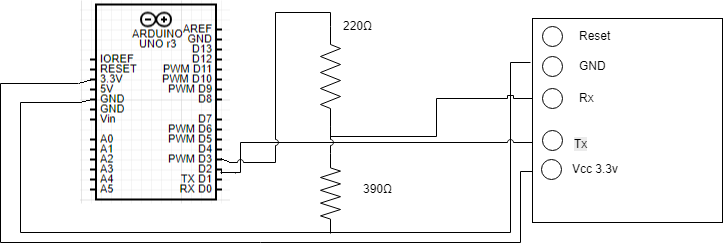
\includegraphics[scale=0.8]{Circuit-Diagram-Wifi-8266}
  \caption{Circuit diagram of the Wifi chip}
  \label{fig:Wifi Circuit}
\end{figure}

\begin{figure}[!ht]
  \centering
      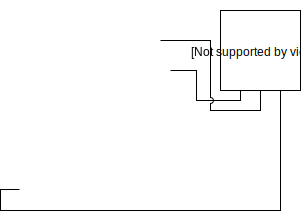
\includegraphics[scale=0.9]{Capacitive}
  \caption{Circuit for Capacitive sensor.}
  \label{fig:CapacitiveCircuit}
\end{figure}

\begin{figure}[!ht]
  \centering
      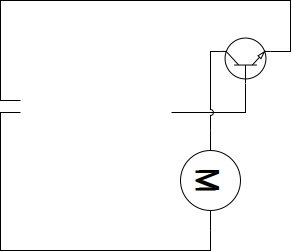
\includegraphics[scale=0.9]{Pumpan}
  \caption{Circuit for water pump.}
  \label{fig:WaterPumpCircuit}
\end{figure}

\begin{figure}[!ht]
  \centering
      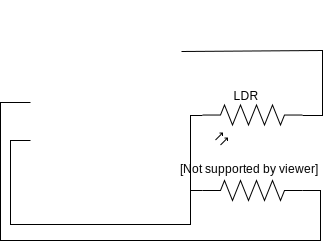
\includegraphics[scale=0.9]{LDR}
  \caption{Circuit for LDR.}
  \label{fig:LDRCircuit}
\end{figure}

\begin{figure}[!ht]
  \centering
      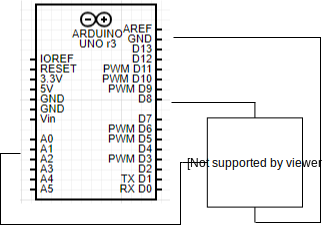
\includegraphics[scale=0.9]{Arduinoxml}
  \caption{Circuit for TMP Sensor}
  \label{fig:TMP36GZCircuit}
\end{figure}


\chapter{Arduino Components}
The following are pictures of our sensors and other components.

\section{fc-28}
\begin{figure}[!ht]
  \centering
      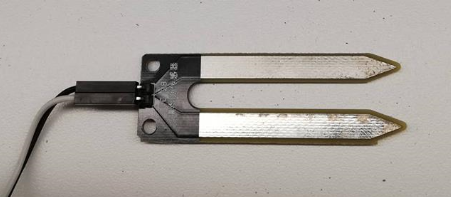
\includegraphics{fc-28-corrosion}
  \caption{Corroded fc-28 after moderate use.}
  \label{fig:resistive}
\end{figure}

\section{Pump}
\begin{figure}[ht!]
	\begin{itemize}
	\item 100\% brand new and high quality
	\item DC Voltage:2.5-6V
	\item Maximum lift:40-110cm / 15.75"-43.4"
	\item Flow rate:80-120L/H
	\item Outside diameter of water outlet: 7.5mm / 0.3"
	\item Inside diameter of water outlet: 4.7mm / 0.18"
	\item Diameter:Approx. 24mm / 0.95"
	\item Length:Approx. 45mm / 1.8"
	\item Height:Approx. 33mm / 1.30"
	\item Material:engineering plastic
	\item Driving mode: brushless dc design, magnetic driving
	\item Continuous working life of 500 hours
	\end{itemize}
	\label{fig:pump description}
\end{figure}

\section{ESP-01}
\begin{figure}[!ht]
	\centering
		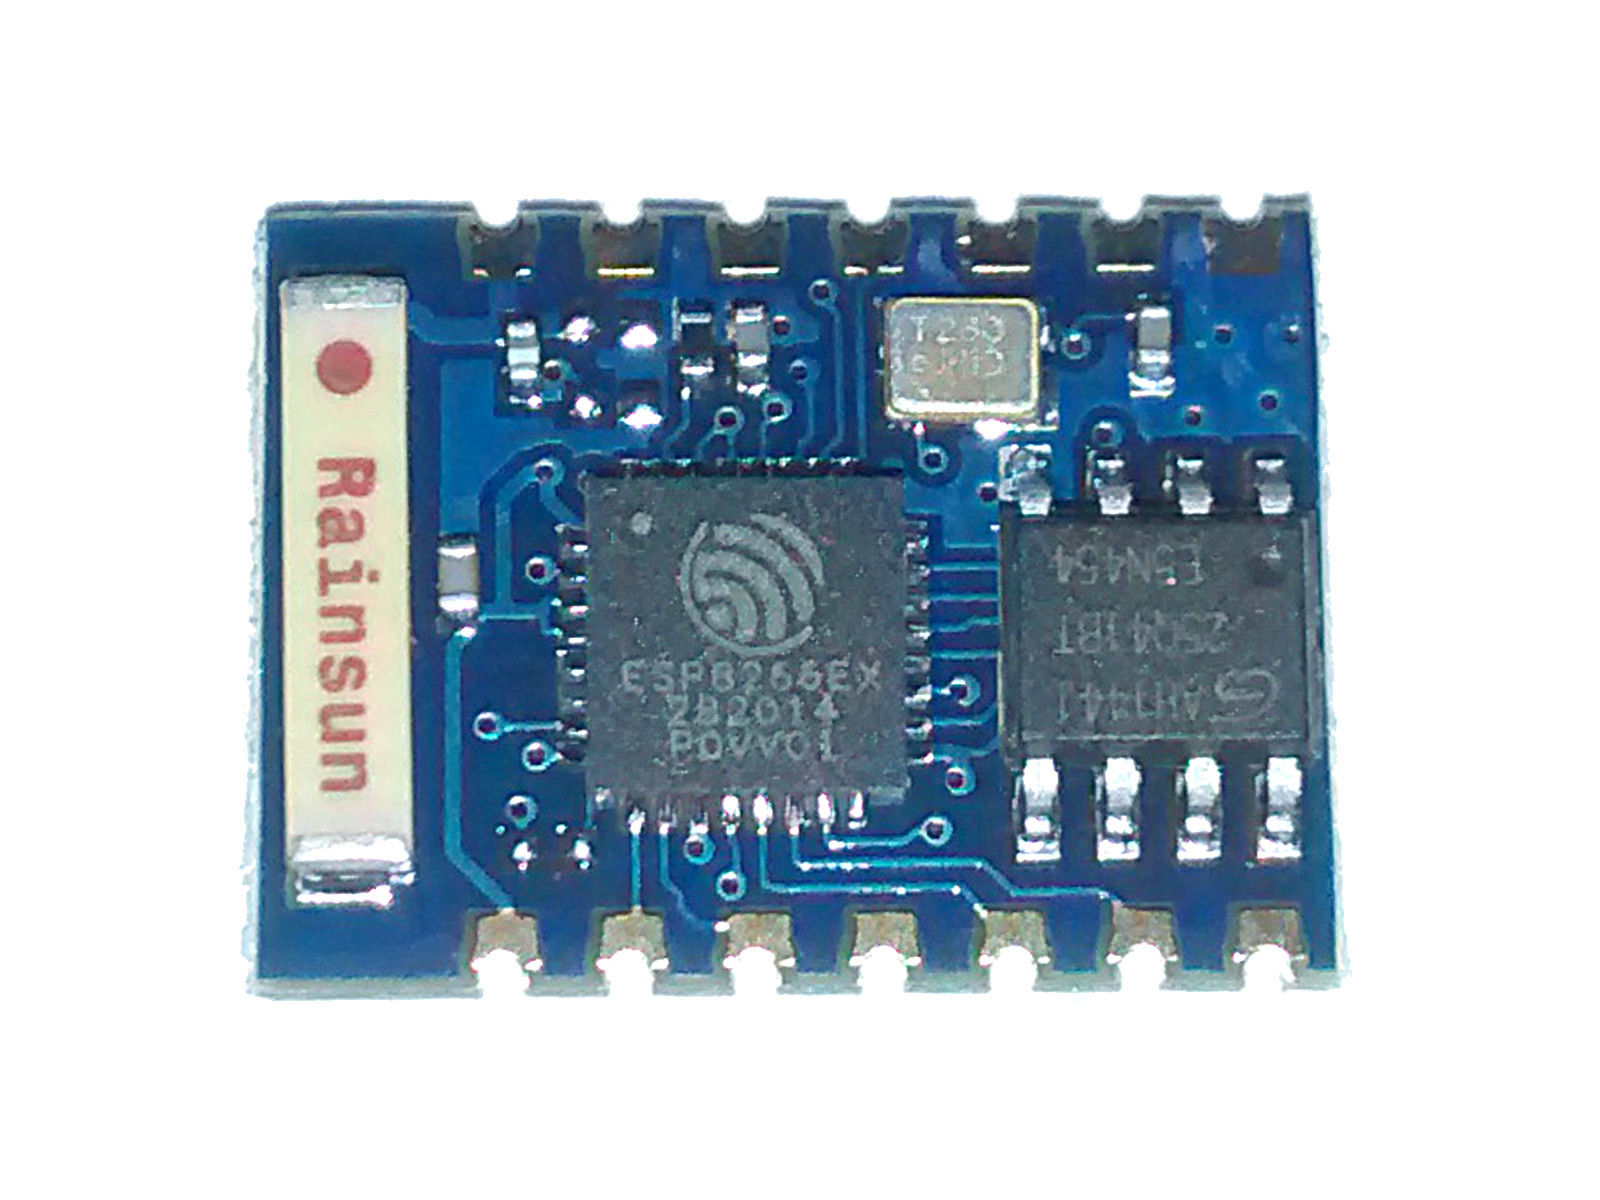
\includegraphics[scale=0.20]{ESP-01}
	\caption{ESP8266-01 module. You can see that distance between each pin is small which meant for us that it was hard to sold for someone inexperienced}
	\label{fig:ESP}
\end{figure}

\chapter{Latex Listings}
The code highlighting in this tex document was taken from \href{https://github.com/trihedral/ArduinoLatexListing/blob/master/arduinoLanguage.tex}{trihedral's ArduinoLatexListing Github repository}

\section{Ardunio Ino File}
\begin{lstlisting}[caption={Arduino Code Main}\label{list:ArduinoMain}, language=Arduino]
#include "ESP8266.h"
#include "CapacitiveMoistureSensor.h"
#include "LightSensor.h"
#include "TemperatureSensor.h"
#include <SoftwareSerial.h>

/*
   Definitions
*/
#define SSID        "Kristmund Hotspot"
#define PASSWORD    "skopun240"
#define HOST_NAME   "192.168.137.163"
#define HOST_PORT   (8080)

/*
   Declarations
*/
SoftwareSerial mySerial(2, 3); /* RX:D4, TX:D3 */
ESP8266 wifi(mySerial, 115200);
uint32_t len;

void setup() {
  //Init debug serial connection
  Serial.begin(9600);
  Serial.println("Serial connection setup [DONE]");
  Serial.println("Allowing ESP8266 time to start...");
  delay(10000);
 

  //Init WiFi
  while (true) {
    Serial.println("WiFi setup [START]");
    if (wifi.joinAP(SSID, PASSWORD)) {
      Serial.print("Join AP success\r\n");
      if (wifi.disableMUX()) {
        Serial.println("WiFi setup [DONE]");
        break;
      } else {
        Serial.println("WiFi setup [MUX ERR]");
      }
    } else {
      Serial.println("WiFi setup [AP ERR]");
    }
    //If init failed, wait 20s and try again
    delay(20000);
  }
  while (true) {
    if (wifi.createTCP(HOST_NAME, HOST_PORT)) {
      break;
    }
    else {
      Serial.println("Create tcp [ERR]");
      delay(10000);
    }
  }

  Serial.println(wifi.getVersion());
  Serial.println(wifi.getAPList());
}

struct Data {
  public:
    uint16_t plantId;
    uint8_t temperature;
    uint8_t moisture;
    uint32_t light;
    uint8_t water;
};

struct Package {
  union {
    Data values;
    uint8_t bytes[9];
  } data;
};

class DataHandler {
  private:
    const uint16_t plantId = 1;
    Package package;
    const CapacitiveMoistureSensor moisture = CapacitiveMoistureSensor(4, A2);
    const TemperatureSensor temperature = TemperatureSensor(8, A1);
    const LightSensor light = LightSensor(13, A0);

    void populatePackage() {
      Data& values = package.data.values;
      values.plantId = this->plantId;
      values.temperature = temperature.read();
      values.moisture = moisture.read();
      values.light = light.read();
      values.water = 90;
    }

  public:
    DataHandler() {
    }
  public:
    const Package& getPackage() {
      populatePackage();
      return package;
    }
};

const DataHandler dataHandler;

void loop() {
  Package package = dataHandler.getPackage();
  
  while (!wifi.send(package.data.bytes, sizeof(package.data.bytes))) {
    Serial.println("Send data [ERR]");
  }
  Serial.println("Send data [YESMAN]");
  
  
  delay(5000);
}
\end{lstlisting}

\section{Light Reading}
\begin{lstlisting}[caption={lightReading}\label{list:LightReading}, language=Arduino]
uint32_t LightSensor::read() {
  Serial.println("Reading LIGHT");
  digitalWrite(dPin,HIGH);
  delay(1000);
  uint32_t read = analogRead(aPin);
  digitalWrite(dPin,LOW);
  return read;
}
\end{lstlisting}

\section{Models}
\begin{lstlisting}[caption={models}\label{list:Models}, language=CSharp]
public class ArduinoData
{
	public int Temperature { get; set; }
	public uint Moisture { get; set; }
	public Plant Plant { get; set; }
	public uint PlantId { get; set; }
	[Key]
    public long DataId { get; set; }
	public int Light { get;  set; }
	public int Water { get;  set; }
}

public class Plant
{
	public long PlantId { get; set; }
    public string Name { get; set; }
	public DateTime DateAdded { get; set; }
	public ApplicationUser ApplicationUser { get; set; }
	public IList<ArduinoData> Datas { get; set; }
}

public class ApplicationUser : IdentityUser
{
	public string Name { get; set; }
	public virtual List<Plant> Plants { get; set; }  
}
\end{lstlisting}
\section{Abstract Interfaces}
\begin{lstlisting}[caption={Interfaces}\label{list:Interfaces},language=CSharp]
public interface IArduinoDataRepository
{
	void SaveData(ArduinoData data);
}

public interface IPlantRepository
{
	Task<IEnumerable<Plant>> UserPlants();
    Task SavePlant(Plant plant);
}

public interface IEGardenerContext
{
	DbSet<Plant> Plants { get; set; }
} 

public interface IUserRepository
{
	ApplicationUser GetCurrentUser();
}
\end{lstlisting}
\section{EGarden Context}
\begin{lstlisting}[caption={EGardenerContext}\label{list:EGardengerContext},language=CSharp]
 public class EGardenerContext : IdentityDbContext<ApplicationUser,IdentityRole,string>,
						IEGardenerContext
    {

        public EGardenerContext(DbContextOptions options)
            : base(options)
        {
        }

        //public DbSet<User> Users { get; set; }
        public DbSet<Plant> Plants { get; set; }


        protected override void OnModelCreating(ModelBuilder builder)
        {
            base.OnModelCreating(builder);
        }

        public EGardenerContext CreateDbContext(string[] args)
        {
            //optionsBuilder.UseSqlServer(
            "Server=.\\SQLEXPRESS;Database=EGarden; user id=sa;
            password=Password0;Trusted_Connection=False;
            MultipleActiveResultSets=true;");

            return new 
            EGardenerContext(
            newDbContextOptionsBuilder<EGardenerContext>()
                .UseSqlServer(
                    "Server=(localdb)
                    mssqllocaldb;Database=E.Gardener;
                    Trusted_Connection=True;
                    MultipleActiveResultSets=true")
                .Options);
        }
    }
}

\end{lstlisting}
\section{ArduinoDataLoggerRepository}
\begin{lstlisting}[caption={EFDataLoggerPlantRepository}\label{list:EFDataLoggerPlantRepository},language=CSharp]
public class EFDataLoggerPlantRepository
{
	private readonly EGardenerContext _context;

	public	EFDataLoggerPlantRepository(
	EGardenerContext context)
	{
       _context = context;
	}


	public void SavePlantData(ArduinoData data)
	{
		var plantQueryable = _context.Plants
			.Include(x => x.Datas);
             var plant = plantQueryable.Single(x=>
             x.PlantId == data.PlantId);
             
		plant.Datas.Add(data);
		_context.SaveChanges();
	}
}
\end{lstlisting}

\section{Observer Code}
\begin{lstlisting}[caption={Observer Class}\label{list:Observer}, language=CSharp]
public class Observer : IObserver<ArduinoData>, IDisposable
{
	private IDisposable _unsubscriber;
    private readonly EFDataLoggerPlantRepository _arduinoDataRepository;

	  public Observer()//, IObservable<ArduinoData> observable)
        {
            _arduinoDataRepository = new EFDataLoggerPlantRepository(new
            EGardenerContext(
                new DbContextOptionsBuilder()
                   .UseSqlServer("Server=127.0.0.1;Database=EGarden;
                   User Id=SA;Password=Password0").Options)
            );
        }

	public void Subscribe(IObservable<ArduinoData> provider)
    {
		if (provider != null)
		{	     
	        _unsubscriber = provider.Subscribe(this);
        }
	}
	public void OnCompleted()
    {
		Console.WriteLine($"connection to  closed.");
	    this.Unsubscribe();
    }

	public void OnError(Exception e)
	{
        Console.WriteLine($": Error in connection or transmission of data.");
	}

    // This runs when data from arduino is received.
	public void OnNext(ArduinoData value)
    {
       _arduinoDataRepository.SavePlantData(value);
    }

    public void Unsubscribe()
	{
        _unsubscriber.Dispose();
	}

	public void Dispose()
    {
		_unsubscriber?.Dispose();
	}
}
\end{lstlisting}

\begin{lstlisting}[caption={Observable Class}\label{list:Observable}, language=CSharp]
public class Observable : IDisposable, IObservable<ArduinoData>, IHostedService
{
	private const int Port = 8080;
    private readonly TcpListener _socket;
    private List<IObserver<ArduinoData>> Observers { get; }

	public Observable(IServiceProvider serviceProvider)
	{
	//prep
		Observers = new List<IObserver<ArduinoData>>();
		_socket = new TcpListener(IPAddress.Any, Port);
                
		// subscribing necessary observers
		serviceProvider.GetService<Observer>().Subscribe(this);
        serviceProvider.GetService<DataPusherObserver>().Subscribe(this);
	}

	private void Listen()
	{
		while(true)
		{
			var client = _socket.AcceptTcpClient();
		    new Thread(() => ListenToClient(client)).Start();
   		}
	}

	private void ListenToClient(TcpClient client) {
        while(client.Connected)
        {
			var reader = client.GetStream();
            while(client.Available > 0)
            {
			// while(reader.DataAvailable)\\
			 {
				byte[] buffer = new byte[2];
                var data = new ArduinoData();

                reader.Read(buffer,0,2);
				data.PlantId = BitConverter.ToUInt16(buffer);
				data.Temperature = reader.ReadByte();
                    
                data.Moisture = (uint) reader.ReadByte();
                    
				buffer = new byte[4];
                    
                reader.Read(buffer,0,4);
                data.Light = BitConverter.ToInt32(buffer);
                data.Water = reader.ReadByte();
                   
                Notify(data);
              }
                Thread.Sleep(1000);
            }
            client.Close();
       }


	public void Dispose()
    {
		 // closing 
	    _socket.Stop();

		foreach (var observer in Observers.ToArray())
			if (Observers.Contains(observer))
				observer.OnCompleted();

            Observers.Clear();
        }


	public IDisposable Subscribe(IObserver<ArduinoData> observer)
	{
		if (!Observers.Contains(observer))
				Observers.Add(observer);
           
            return new Unsubscriber(Observers, observer);
    }

	private class Unsubscriber : IDisposable
	{
		private readonly List<IObserver<ArduinoData>> _observers;
	    private readonly IObserver<ArduinoData> _observer;

        public Unsubscriber(List<IObserver<ArduinoData>> observers,
        						 IObserver<ArduinoData> observer)
		{
			this._observers = observers;
			this._observer = observer;
		}
		
		public void Dispose()
		{
			if (_observer != null && _observers.Contains(_observer))
					_observers.Remove(_observer);
        }
	}

	public void Notify(ArduinoData data)
	{
		if (data.PlantId == 21569)
		{
			Console.WriteLine("something something id invalid..-");
            return;
		}
            
		foreach (var observer in Observers)
		{
			if (data == null)
				observer.OnError(new Exception("Notifying corrupt data from
				arduino"));
			else
			{
				try
				{
					observer.OnNext(data);
				}catch (InvalidOperationException exception)
				{
                        // TODO: ...
					Console.WriteLine(exception.Message);
				}

			}
		}
	}

	public Task StartAsync(CancellationToken cancellationToken)
	{
		_socket.Start();
	    new Thread(Listen).Start();
        return Task.CompletedTask;
	}

	public Task StopAsync(CancellationToken cancellationToken)
	{
		Dispose();
	    return Task.CompletedTask;
    }
}
\end{lstlisting}

\begin{lstlisting}[caption={Datapusher.js Class}\label{list:DatapusherJs}, language=CSharp]
const connection = new signalR.HubConnectionBuilder().withUrl("/dataHub")
													.build();

connection.on("UpdateData", function (data) {
    console.log(data);
    const plantDiv = document.getElementById(data.plantId);

    plantDiv.getElementsByClassName("id")[0]
        .getElementsByClassName("value")[0]
        .textContent = data.dataId;
 
    plantDiv.getElementsByClassName("temperature")[0]
        .getElementsByClassName("value")[0]
        .textContent = data.temperature;

    plantDiv.getElementsByClassName("moisture")[0]
        .getElementsByClassName("value")[0]
        .textContent = data.moisture;

    plantDiv.getElementsByClassName("light")[0]
        .getElementsByClassName("value")[0]
        .textContent = data.light;

    plantDiv.getElementsByClassName("water")[0]
        .getElementsByClassName("value")[0]
        .textContent = data.water;
});

connection.start().catch(function (err) {
    return console.error(err.toString());
});
\end{lstlisting}
\begin{lstlisting}[caption={HomeController}\label{list:HomeController}, language=CSharp]

public class HomeController : Controller
{
	private readonly IPlantRepository _plantRepository;
    private readonly IApplicationUserAccessor _userAccessor;


	public HomeController(IPlantRepository repository,
						 IApplicationUserAccessor userAccessor)
	{
		_plantRepository = repository;
	    _userAccessor = userAccessor;
    }

	[Authorize]
	public async Task<IActionResult> Index()
    {
            
	return View(await _plantRepository.UserPlants());
    }

	public async Task<string> UpdateName()
	{
		await _plantRepository.SavePlant(new Plant()
		{
	        Name = "hey"
        });
        return _plantRepository.UserPlants().ToString();
	}

	public async Task<IActionResult> About()
    {
		ViewData["Message"] = "Description of your profile";

		var user = await _userAccessor.User;

	    return View(user);
    }
        
	[ResponseCache(Duration = 0, Location = ResponseCacheLocation.None,
					 NoStore = true)]        
	public IActionResult Error()
	{
		return View(new ErrorViewModel { RequestId = Activity.Current?.Id ??
	    HttpContext.TraceIdentifier });
   }
}
\end{lstlisting}

\begin{lstlisting}[caption={IndexView}\label{list:IndexView}, language=HTML]
@model IEnumerable<Repository.Models.Plant>

<div align="center">
    <table class="table table-condensed">
        <tr>
            <th>Plant ID</th>
            <th>Name</th>
            <th>Added</th>
        </tr>
        <tr>
        </tr>
        @foreach (var plant in Model)
        {
            <tr>
                <td>@plant.PlantId</td>
                <td>@plant.Name</td>
                <td>@plant.DateAdded</td>
            </tr>
        }
    </table>
</div>
\end{lstlisting}

\begin{lstlisting}[caption={AboutView}\label{list:AboutView}, language=HTML]
@model Repository.Models.ApplicationUser;

<h2>Your Profile Description</h2>
<p>Login user name: @Model.Name</p>
@{
    if (Model.Plants == null)
    {
        <p>Number of Plants: 0</p>
    }
    else
    {
        <p>Number of Plants: @Model.Plants.Count</p>
    }

    if (!Model.PhoneNumberConfirmed)
    {
        <p>No phone number attached to this user.
         You can add it by pressing
         your user name in the top right corner</p>
    }
    else
    {
        <p>Phone Number: @Model.PhoneNumber</p>
    }
}


\end{lstlisting}
\begin{lstlisting}[caption={PlantController}\label{list:PlantController}, language=CSharp]

[Authorize]
public class PlantController : Controller
{
    private readonly IPlantRepository _repository;

	public PlantController(IPlantRepository repository)
    {
       _repository = repository;
	}
        
        
    public async Task<IActionResult> Index()
	{   
        return View(await _repository.UserPlants());
	}

    public async Task<IActionResult> Add(Plant plant)
	{
        if (plant != null && ModelState.IsValid)
	    {
		await _repository.SavePlant(plant);
        return await Index();
		}   

        return View(plant);            
	}


	public PartialViewResult PlantPartial(Repository.Models.Plant plant)
    {    
	return PartialView("_plant_partial", plant);
    }

	public async Task<PartialViewResult> PlantsPartial()
    {
        return PartialView("_plants_partial",await _repository.UserPlants());
	}
}
\end{lstlisting}
\backmatter 
\cleardoublepage\addcontentsline{toc}{chapter}{Bibliography}
\bibliographystyle{plainnat}
\bibliography{bibliography}
\end{document}
